\begin{figure*}[h!]\centering
    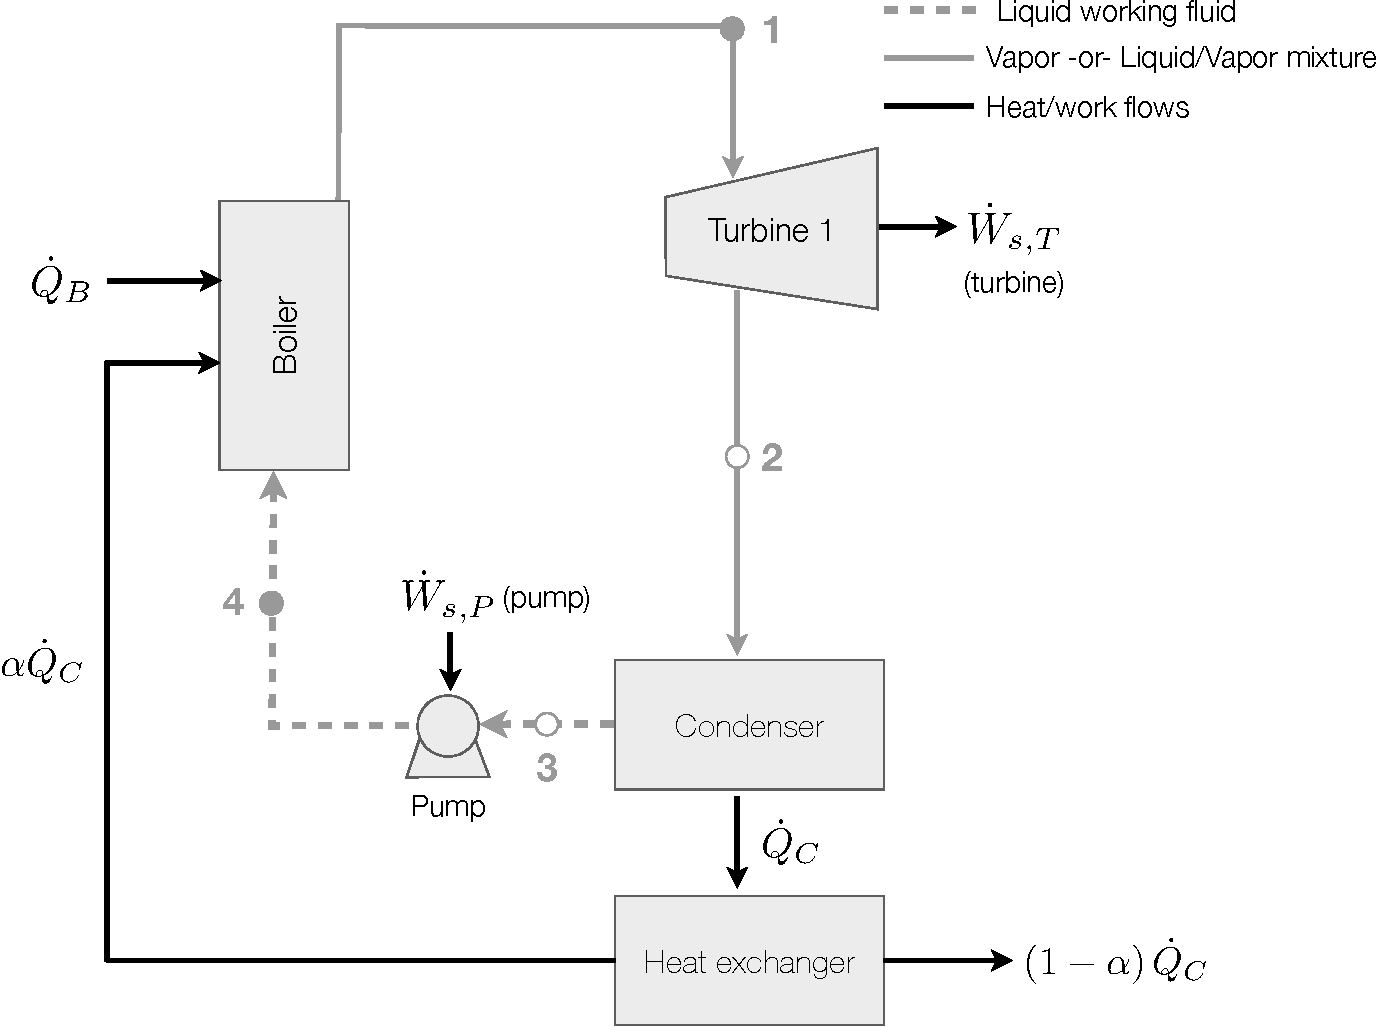
\includegraphics[width=0.72\textwidth]{./figs/Fig-Mod-Rankine-ENGRI-1120-F22.pdf}
    \caption{Schematic of the unit operations of a modified organic Rankine cycle in which a fraction of the heat from the condenser is recycled to the boiler through a heat exchanger.}\label{fig-rankine-cycle}
    \end{figure*}
    
    \item{(30 pt)~The Organic Rankine Cycle (ORC) is an \textit{open} four step thermodynamic process used to generate power that uses organic compounds as 
    working fluids (Fig. \ref{fig-rankine-cycle}). In the cycle, path $\mathcal{P}_{ij}$ connects operating point $\mathcal{O}_{i}$ to $\mathcal{O}_{j}$:
    \begin{itemize}
      \item[$\mathcal{P}_{41}$]{$\left(4~\rightarrow~1\right)$: \textit{isobaric} heating in a boiler from operating point $\mathcal{O}_{4}$ to $\mathcal{O}_{1}$}
      \item[$\mathcal{P}_{12}$]{$\left(1~\rightarrow~2\right)$: \textit{adiabatic} expansion in a turbine from operating point $\mathcal{O}_{1}$ to $\mathcal{O}_{2}$}
      \item[$\mathcal{P}_{23}$]{$\left(2~\rightarrow~3\right)$: \textit{isobaric} cooling in a condenser from operating point $\mathcal{O}_{2}$ to $\mathcal{O}_{3}$}
      \item[$\mathcal{P}_{34}$]{$\left(3~\rightarrow~4\right)$: \textit{adiabatic} compression in a pump from operating point $\mathcal{O}_{3}$ to $\mathcal{O}_{4}$}
    \end{itemize}

    \textbf{Nomenclature}: $\dot{W}_{s,T}$ denotes the rate of turbine shaft work (units: kJ s$^{-1}$); 
    $\dot{W}_{s,P}$ denotes the rate of pump shaft work (units: kJ s$^{-1}$); 
    $\dot{Q}_{B}$ denotes the rate of heat input/output to/from the boiler (units: kJ s$^{-1}$);
    $\dot{Q}_{C}$ denotes the rate of heat input/output to/from the condenser (units: kJ s$^{-1}$)
    
    \textbf{Assume}: (i) the cycle operates at steady-state; (ii) the working fluid (HFC-134A) has a mass flow rate of $\dot{m}$ = 2.25 kg s$^{-1}$;
    (iii) \textit{neglect} the enthalpy and temperature change from the pump (assume T$_{3}\simeq$~T$_{4}$ and H$_{3}\simeq$~H$_{4}$);
    (iv) neglect changes in the kinetic and potential energy in the system and streams; (v) the turbine efficiency $\eta_{T}$ = 85\%.
    
    \begin{itemize}
      \item[a)]{(12 pt)~Compute the missing state values in Table \ref{tbl-rankine-simple-state}.}
      \item[b)]{(12 pt)~Compute the missing values in Table \ref{tbl-rankine-simple-work} without heat recycle ($\alpha$ = 0).}
      \item[c)]{(3 pt)~Compute the ideal organic Rankine cycle efficiency: $\eta$ = $-\dot{W}_{net}$/$\dot{Q}_{B}$ if there is no heat recycle ($\alpha$ = 0).}
      \item[d)]{(3 pt)~Compute the ideal organic Rankine cycle efficiency if $\alpha$ = 0.33. Does the efficiency increase, decrease or stay the same when compared with c)?}
    \end{itemize}
    
    \clearpage
    
    \begin{table}[!ht]
      \centering
      \caption{State table for the ideal Rankine cycle problem with heat recycle.}\label{tbl-rankine-simple-state}
    
      \renewcommand{\arraystretch}{2.0}
      \setlength{\tabcolsep}{14pt}
      \begin{tabular}{c|c|c|c|c|c}\toprule
      $\mathcal{O}$ & T ($^{\mathrm{o}}$C) & P (MPa/kPa) & H (kJ kg$^{-1}$) & S (kJ kg$^{-1}$ K$^{-1}$) & Quality $\theta$ \\ \bottomrule
      $\mathcal{O}_{1}$ & 80.0 & 2.0 MPa & & 1.75 & 1.0 \\ \hline
      $\mathcal{O}_{2}$ &  & 29.41 kPa &  & 1.75 &  \\ \hline
      $\mathcal{O}_{3}$ & & & & & \\ \hline
      $\mathcal{O}_{4}$ & & & & 0.7428 & 0.0 \\ \bottomrule
      \end{tabular}
    \end{table}
    
    \clearpage
    
    \begin{table}[!ht]
      \centering
      \caption{Heat and work table for the Rankine cycle problem with heat recycle ($\alpha$ = 0).}\label{tbl-rankine-simple-work}
    
      \renewcommand{\arraystretch}{2.0}
      \setlength{\tabcolsep}{14pt}
      \begin{tabular}{c|c|c|c}\toprule
      Path & $\dot{Q}$ (kW) & (ideal)~$\dot{W}_{s}$ (kW) & (actual)~$\dot{W}^{*}_{s}$ (kW)\\ \bottomrule
      $\mathcal{P}_{12}$ & 0 & &  \\\hline
      $\mathcal{P}_{23}$ &  & 0 & 0 \\\hline
      $\mathcal{P}_{34}$ & N/A & N/A & N/A \\\hline
      $\mathcal{P}_{41}$ &  & 0 & 0 \\\bottomrule
      Cycle & & & N/A \\\bottomrule
      \end{tabular}
    \end{table}
      
    \clearpage
    }    